\documentclass[dvisvgm,border=0pt]{standalone}
\usepackage[T1]{fontenc}
\usepackage{newtxtext,newtxmath}
\usepackage{tikz}
\usetikzlibrary{arrows.meta,decorations.pathmorphing}

\definecolor{Navy}{HTML}{08154F}
\definecolor{Ink}{HTML}{2B5098}
\definecolor{Blue}{HTML}{315EDB}
\definecolor{BlueTint}{HTML}{DCEBFC}
\definecolor{Sage}{HTML}{568638}
\definecolor{SageTint}{HTML}{E7F2E1}
\definecolor{Gold}{HTML}{F3B122}
\definecolor{Ice}{HTML}{F3FAFF}
\definecolor{Rule}{HTML}{CAE1FA}
\definecolor{Muted}{HTML}{8B95AA}

\tikzset{
  state/.style={draw=Blue,fill=BlueTint,line width=3bp,rounded corners=10bp},
  operation/.style={draw=Sage,fill=SageTint,line width=3bp,rounded corners=10bp},
  wire/.style={draw=Blue,line width=3bp,line cap=round,line join=round},
  blue arrow/.style={wire,-{Stealth[length=13bp,width=12bp]}},
  gold arrow/.style={draw=Gold,line width=6bp,line cap=round,-{Stealth[length=19bp,width=20bp]}},
  time arrow/.style={draw=Muted,line width=3bp,-{Stealth[length=17bp,width=15bp]}},
}

\newcommand{\figbackground}[2]{
  \path[use as bounding box] (0,0) rectangle (#1,#2);
  \fill[Ice!45] (0,0) rectangle (#1,#2);
}

\newcommand{\figtext}[5][Navy]{
  \node[text=#1,font=\fontsize{#4}{#4}\selectfont,inner sep=0bp,align=center]
    at (#2,#3) {#5};
}

\newcommand{\figmath}[5][Navy]{
  \figtext[#1]{#2}{#3}{#4}{$\displaystyle #5$}
}

\newcommand{\panelheading}[3]{
  \fill[BlueTint] (#1,190) circle (35bp);
  \node[text=Navy,font=\fontsize{40}{42}\selectfont\bfseries,inner sep=0bp]
    at (#1,190) {#2};
  \node[text=Navy,anchor=west,font=\fontsize{40}{42}\selectfont\bfseries,inner sep=0bp]
    at ({#1+62},190) {#3};
}

\newcommand{\panelrules}{
  \draw[Rule,line width=2bp] (535,162) -- (535,733);
  \draw[Rule,line width=2bp] (1090,162) -- (1090,733);
}

\newcommand{\statebox}[4]{
  \fill[Blue,opacity=.08,rounded corners=10bp]
    ({#1+4},{#2+6}) rectangle ({#3+4},{#4+6});
  \draw[state] (#1,#2) rectangle (#3,#4);
}

\newcommand{\operationbox}[4]{
  \fill[Sage,opacity=.08,rounded corners=10bp]
    ({#1+4},{#2+6}) rectangle ({#3+4},{#4+6});
  \draw[operation] (#1,#2) rectangle (#3,#4);
}

\newcommand{\processstrip}[4]{
  \fill[BlueTint!70,rounded corners=20bp] (50,762) rectangle (1622,858);
  \foreach \x/\word in {132/#1,522/#2,912/#3,1302/#4} {
    \fill[BlueTint,rounded corners=15bp] (\x,781) rectangle ({\x+306},837);
    \node[text=Navy,font=\fontsize{30}{34}\selectfont\bfseries,inner sep=0bp]
      at ({\x+153},809) {\word};
  }
  \foreach \x in {465,855,1245} {
    \draw[gold arrow] (\x,809) -- ({\x+31},809);
  }
}


\begin{document}
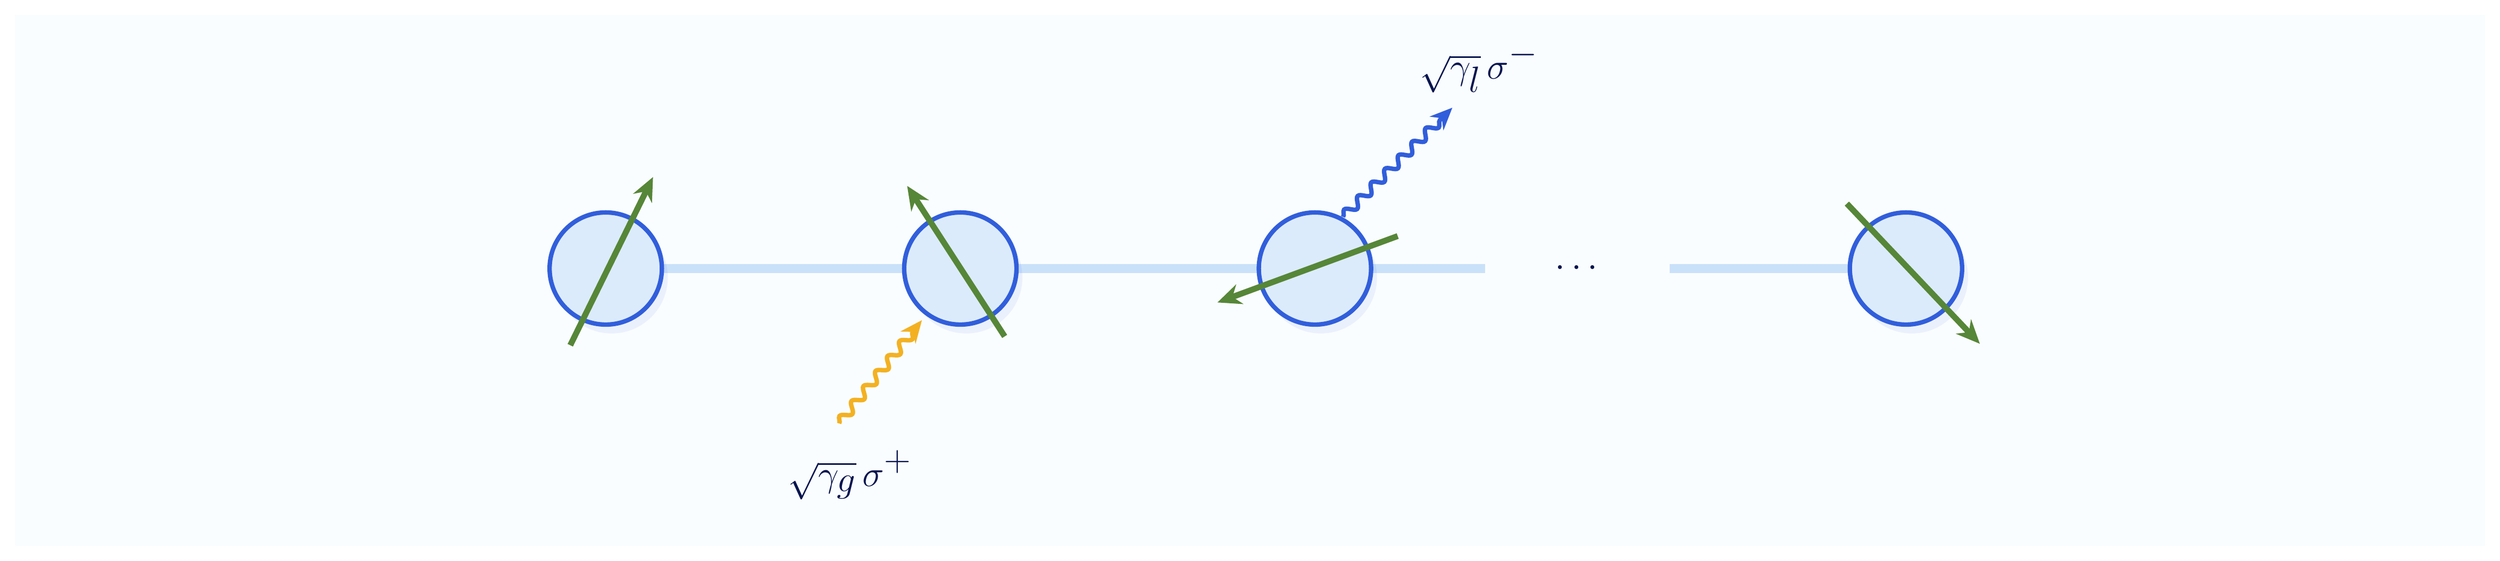
\begin{tikzpicture}[x=1bp,y=-1bp]
  \figbackground{1672}{360}

  % Preserve the spin-chain, gain, and loss content of the original schematic.
  \draw[Rule,line width=6bp] (400,172) -- (880,172);
  \draw[Rule,line width=6bp] (880,172) -- (995,172);
  \draw[Rule,line width=6bp] (1120,172) -- (1280,172);
  \figmath{1057}{172}{35}{\cdots}
  \foreach \x in {400,640,880,1280} {
    \fill[Blue,opacity=.08] (\x+4,178) circle (38bp);
    \draw[draw=Blue,fill=BlueTint,line width=3bp] (\x,172) circle (38bp);
  }
  \draw[draw=Sage,line width=4bp,-{Stealth[length=16bp,width=14bp]}]
    (376,224) -- (432,110);
  \draw[draw=Sage,line width=4bp,-{Stealth[length=16bp,width=14bp]}]
    (670,218) -- (604,116);
  \draw[draw=Sage,line width=4bp,-{Stealth[length=16bp,width=14bp]}]
    (936,150) -- (814,195);
  \draw[draw=Sage,line width=4bp,-{Stealth[length=16bp,width=14bp]}]
    (1240,128) -- (1330,223);
  \draw[draw=Gold,line width=3bp,decorate,
    decoration={snake,amplitude=3bp,segment length=13bp,post length=7bp},
    -{Stealth[length=15bp,width=13bp]}] (558,277) -- (614,207);
  \draw[draw=Blue,line width=3bp,decorate,
    decoration={snake,amplitude=3bp,segment length=13bp,post length=7bp},
    -{Stealth[length=15bp,width=13bp]}] (899,137) -- (973,63);
  \figmath{565}{312}{44}{\sqrt{\gamma_g}\,\sigma^+}
  \figmath{991}{36}{44}{\sqrt{\gamma_l}\,\sigma^-}
\end{tikzpicture}
\end{document}
